\documentclass[a4paper, 10 pt]{article}

\usepackage[a4paper,bindingoffset=0.2in,%
left=3cm,right=3cm,top=2.5cm,bottom=2.5cm,%
footskip=.25in]{geometry}

% IDIOMA
\usepackage[english]{babel} 

% ENCODING
\usepackage{cmap,lmodern,hyperref}
\usepackage[T1]{fontenc}
\usepackage[utf8]{inputenc}
%\usepackage[bookmarks]{hyperref}

% IMATGES
\usepackage{wrapfig,graphicx}
\usepackage[font=small]{caption}
\usepackage{subcaption}

% EQUACIONS
\usepackage{mathtools,amsmath,amssymb,systeme,braket}

% OTROS
\usepackage{listings,color,enumitem}
%\usepackage{subfiles}
%\usepackage{titlesec, titletoc, blindtext,etoolbox,csquotes}


\setlength{\parindent}{0em}
\setlength{\parskip}{0.3em}
\setlist{noitemsep,nolistsep}
%\graphicspath{../Figures}

\begin{document}
\section*{Troubleshooting}


\subsubsection*{A brief discussion on the binning error and its correction}
\textbf{If you just want to see the results, feel free from skipping this section.}

In our analysis from the DayaBay and NEOS data, the NEOS data is not being significant enough to rule out sterile neutrinos with large masses and intermediate mixing angle.

Carlos correctly noted that there was a mistake with our analysis: we were losing information from the NEOS data because we were averaging every two data points. In order to correct such error, we have kept almost all the data points from NEOS, and modified the analysis such that each nuissance parameters takes into account two bins from NEOS for each bin from DayaBay. That is, NEOS keeps all its data, but these data contribute to the nuissance parameters in pairs. Namely,

\[
\alpha_i = 
\frac{O^{EH1}_i + O^{EH2}_i + O^{EH3}_i + O^{NEOS}_{2i} + O^{NEOS}_{(2i+1)}}{  
P^{EH1}_i + P^{EH2}_i + P^{EH3}_i + P^{NEOS}_{2i} + P^{NEOS}_{(2i+1)}}
\]

This difference on the nuissances may also introduce an error, but since the number of events in NEOS is much more smaller (by 3 orders of magnitude) to those of DayaBay, it should be small.


\textbf{Note}: in fact, not all data points from NEOS have been taken into account. The initial bins, (1.0,1.1), (1.1,1.2), (1.2,1.3); and the final bins (6.9,7.0),(7.0, 10.0) have not been taken into account because it would require for us to interpolate, and I would prefer to discuss things before implementing such interpolation. As we discussed, the initial bins won't bring any problem. The two last bins may, but in my opinion two bins should not introduce such a large discrepancy between our results and Dentler's.

\vspace{0.5cm}
\hrule

\subsubsection*{Results after the correction}
Nevermind, the error has been corrected and now NEOS should be more significant. Or not.

To do so, let's remember the data from Dentler \& Kopp:
\begin{figure}[h]
	\centering
	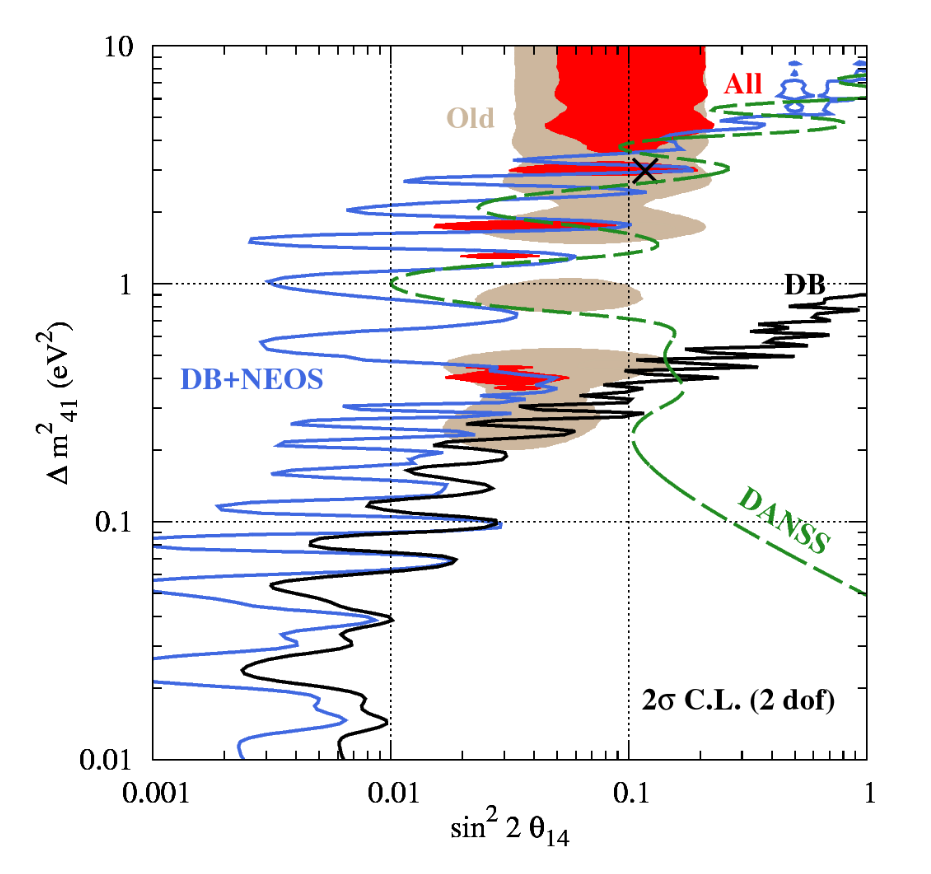
\includegraphics[width=0.6\linewidth]{DentlerKoppParameterSpace}
	\caption{Parameter exclusion according to Dentlet \& Kopp}
	\label{fig:dentlerkoppparameterspace}
\end{figure}


And let's run our analysis for points in this parameter space which are allowed by the DB analysis, and ruled-out by the DB+NEOS analysis. If our analysis is working according to theirs, the NEOS data should rule it out too.

For example, take an sterile with mass 0.6 eV$^2$ and mixing angle $\sin^2 2\theta= 0.06$. In the following plot, we show the ratio of our result to the results from the SM best fit, i.e.
\begin{equation}
R_i = \frac{P_i^{(\text{ste})}}{P_i^{(\text{SM})}}
\end{equation}
 This is a similar plot to 3(c) in [\href{https://arxiv.org/pdf/1709.04294v2.pdf}{1709.04294}]. In the left picture, the errors are purely statistical, according to the following propagation of errors\footnote{Note that the Poisson logarithm does never compute this error. It simply takes into account the number of events.}
 \begin{equation}
 \delta R_i = \frac{\delta P_i^{(\text{ste})}}{P_i^{(\text{SM})}} + \frac{P_i^{(\text{ste})}}{P_i^{(\text{SM})}}\frac{\delta P_i^{(\text{SM})}}{P_i^{(\text{SM})}}\, .
 \end{equation}In the right, the errors are those of the figure 3(c) of  [\href{https://arxiv.org/pdf/1709.04294v2.pdf}{1709.04294}].

\begin{figure}[h]
	\centering
	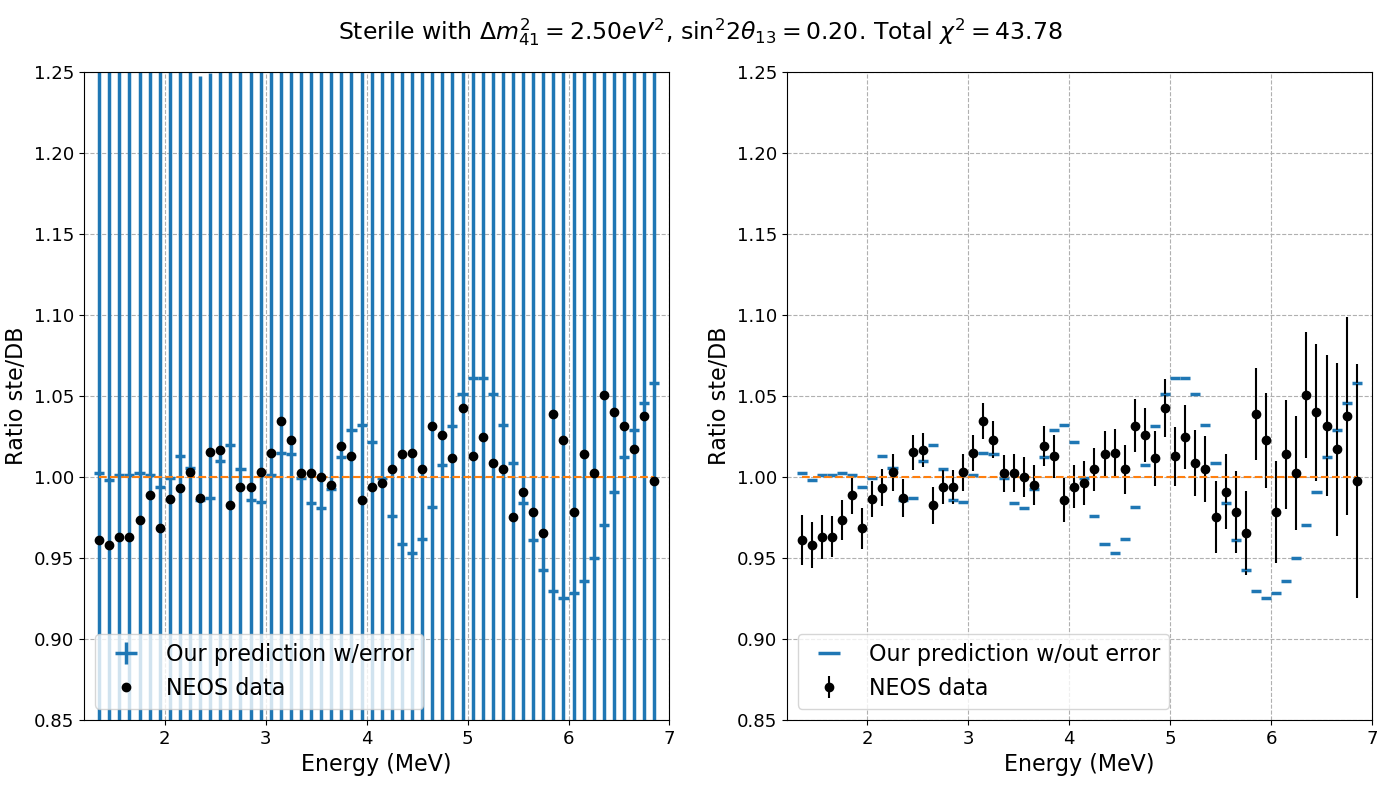
\includegraphics[width=0.7\linewidth]{GlobalFit/Figures/NEOSRatio_2.50_ste}
	\caption{Ratio of the sterile NEOS prediction to the SM NEOS prediction. On the left, statistical errors. On the right, errors from NEOS data.}
	\label{fig:neosratio6}
\end{figure}

As we can see, there is a huge difference between both plots. On the case of the left, the statistical error completely erases any discrepancy between data and expectation. On the case of the right, the error from the data is small and does introduce a discrepancy between data and expectation. On the left, the sterile should not be ruled out. On the right, it probably would.

If you do not feel comfortable with this graphics, let me just plot the event expectation \textit{per se}, for the same mass and mixing:
\begin{figure}[h]
	\centering
	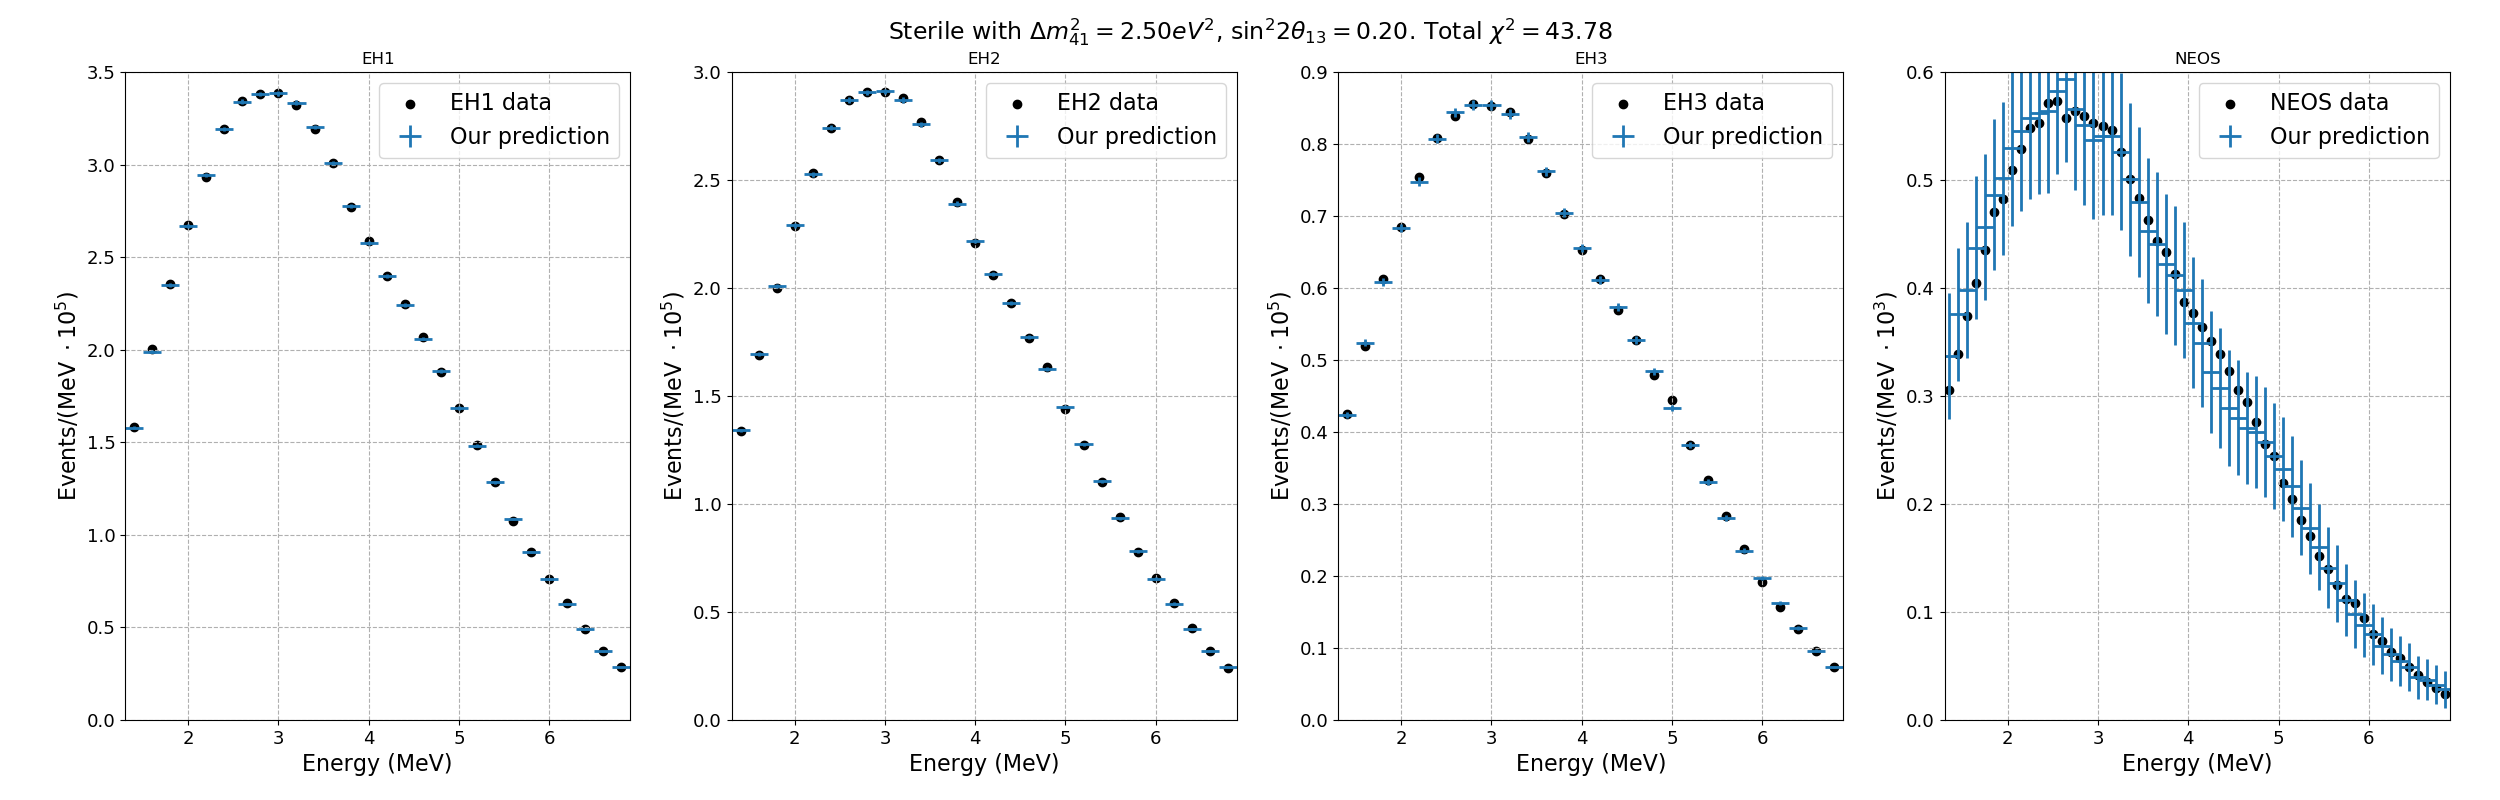
\includegraphics[width=\linewidth]{GlobalFit/Figures/EventExpectation_2.50_ste}
	\caption{Event expectations for an sterile which is ruled-out by Dentler DB+NEOS analysis.}
	\label{fig:eventexpectation2}
\end{figure}

As one can see, the statistical error does accommodate any possible oscillation.

\subsubsection*{Conclusion}
Our Poisson logarithm analysis does not explicitly take into account any statistical nor systematic error. However, it implicitly takes into account that an experiment with fewer data is less significant. In some way, it takes into account statistical error. As we can see, our Poisson logarithm test gives $\chi^2 =42.53$. For reference, the $\chi^2$ from the sterile best fit is $\chi^2 = \textbf{39.16}$. 

{\bfseries Therefore, the procedure we're following would not rule the sterile out. Why? In my opinion, because there is very few data and the statistical error can accommodate any discrepancy. }

My question then is: is our analysis, which uses the Poisson logarithm, correctly implementing NEOS error? 
\end{document}